\documentclass[8pt,a4paper,compress]{beamer}

\usepackage{/home/siyer/lib/slides}

\title{Register Allocation}
\date{}

\begin{document}
\begin{frame}
\vfill
\titlepage
\end{frame}

\begin{frame}
\frametitle{Outline}
\tableofcontents
\end{frame}

\section{Introduction}
\begin{frame}[fragile]
\pause

Register allocation is the process of assigning as many local variables and temporaries to physical registers as possible

\pause
\bigskip

The more values that we can keep in registers instead of memory, the faster our programs will run

\pause
\bigskip

With respect to our LIR, we wish to assign physical registers to each of the virtual registers that serve as operands to instructions

\pause
\bigskip

But there are often fewer physical registers than there are virtual registers

\pause
\bigskip

Sometimes, as program execution progresses, some values in physical registers will have to be spilled to memory while the register is used for another purpose, and then reloaded when those values are needed again

\pause
\bigskip

Code must be generated for storing spilled values and then for reloading those values at appropriate places; we would like to minimize this spilling (and reloading) of values to and from memory
\end{frame}

\begin{frame}[fragile]
\pause

Any register allocation strategy must determine how to most effectively allocate physical registers to virtual registers and, when spilling is necessary, which physical registers to spill to make room for assignment to other virtual registers

\pause
\bigskip

The problem of register allocation is NP-complete in general

\pause
\bigskip

Register allocation that focuses on just a single basic block, or even just a single statement,
is said to be local

\pause
\bigskip

Register allocation that considers the entire flow graph of a method is said to be global

\pause
\bigskip

We will look at a nai\"{i}ve (local) strategy as well as a global strategy based on graph coloring
\end{frame}

\section{Na\"{i}ve Register Allocation}
\begin{frame}[fragile]
\pause

The na\"{i}ve register allocation strategy simply sequences through the operations in the (LIR) code, assigning physical registers to virtual registers

\pause
\bigskip

Once all physical registers have been assigned, and if there are additional virtual registers to deal with, we begin spilling physical registers to memory

\pause
\bigskip

There is no strategy for determining which registers to spill; for example, one might simply sequence through the physical registers a second time in the same order they were assigned the first time, spilling each to memory as it is re-needed

\pause
\bigskip

When a spilled value used again, it must be reloaded into a (possibly different) register

\pause
\bigskip

Such a strategy works just fine when there are as many physical registers as there are virtual registers; in fact, it is as effective as any other register allocation scheme in this case

\pause
\bigskip

When there are many more virtual registers than physical registers, which is always the case, performance of the na\"{i}ve strategy degrades rapidly as physical register values must be repeatedly spilled and reloaded
\end{frame}

\begin{frame}[fragile]
\pause

Following is the SPIM code generated by \jmm using the na\"{i}ve register allocation strategy (and just three physical registers \$t0, \$t1, and \$t2) for \lstinline{Factorial.computeIter()} method

\begin{lstlisting}[language={}]
    subu    $sp,$sp,48 	 # Stack frame is 48 bytes long
    sw      $ra,44($sp) 	 # Save return address
    sw      $fp,40($sp) 	 # Save frame pointer
    sw      $t0,36($sp) 	 # Save register $t0
    sw      $t1,32($sp) 	 # Save register $t1
    sw      $t2,28($sp) 	 # Save register $t2
    addiu   $fp,$sp,44 	 # Save frame pointer

Factorial.computeIter.0:

Factorial.computeIter.1:
    li $t0,1
    sw $t0,0($sp)
    move $t1,$a0
    sw $t1,8($sp)
    lw $t0,0($sp)
    move $t2,$t0
    sw $t2,16($sp)

Factorial.computeIter.2:
    li $t0,0
    sw $t0,4($sp)
    lw $t1,8($sp)
    lw $t0,4($sp)
    ble $t1,$t0,Factorial.computeIter.4
    j Factorial.computeIter.3

\end{lstlisting}
\end{frame}

\begin{frame}[fragile]
\pause

\begin{lstlisting}[language={}]
Factorial.computeIter.3:
    li $t1,-1
    sw $t1,12($sp)
    lw $t1,8($sp)
    lw $t1,12($sp)
    add $t2,$t1,$t1
    sw $t2,20($sp)
    lw $t2,16($sp)
    lw $t1,8($sp)
    mul $t0,$t2,$t1
    sw $t0,24($sp)
    lw $t0,24($sp)
    move $t2,$t0
    sw $t2,16($sp)
    lw $t2,20($sp)
    move $t1,$t2
    sw $t1,8($sp)
    j Factorial.computeIter.2

Factorial.computeIter.4:
    lw $t2,16($sp)
    move $v0,$t2
    j Factorial.computeIter.restore

Factorial.computeIter.restore:
    lw      $ra,44($sp) 	 # Restore return address
    lw      $fp,40($sp) 	 # Restore frame pointer
    lw      $t0,36($sp) 	 # Restore register $t0
    lw      $t1,32($sp) 	 # Restore register $t1
    lw      $t2,28($sp) 	 # Restore register $t2
    addiu   $sp,$sp,48 	 # Pop stack
    jr      $ra 	 # Return to caller
\end{lstlisting}
\end{frame}

\section{Register Allocation by Graph Coloring}
\begin{frame}[fragile]
\pause

Global register allocation works with a method's entire control-flow graph to map virtual registers to physical registers

\pause
\bigskip

One wants to minimize spills to memory; where spills are necessary, one wants to avoid using them within deeply nested loops

\pause
\bigskip

The basic tool in global register allocation is the liveness interval, the sequence of instructions for which a virtual register holds a meaningful value

\pause
\bigskip

A liveness interval for a virtual register extends from the first instruction that assigns it a value to the last instruction that uses its value

\pause
\bigskip

A more accurate liveness interval has ``holes'' in the sequence, where a virtual register does not contain a useful value; for example, a hole occurs from where the previously assigned value
was last used (or read) to the next assignment (or write) of a new value
\end{frame}

\begin{frame}[fragile]
\pause

Consider the control-flow graph for \lstinline{Factorial.computeIter()}
\begin{center}
\visible<2->{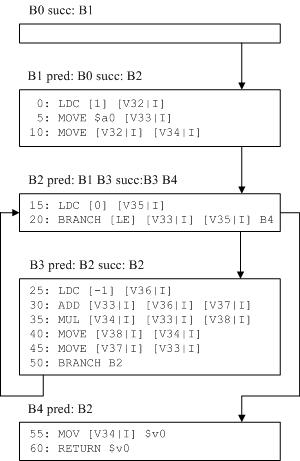
\includegraphics[scale=0.6]{{figures/figure07.01}.jpg}}
\end{center}
\end{frame}

\begin{frame}[fragile]
\pause

The liveness intervals for the above code are illustrated in the following figure
\begin{center}
\visible<2->{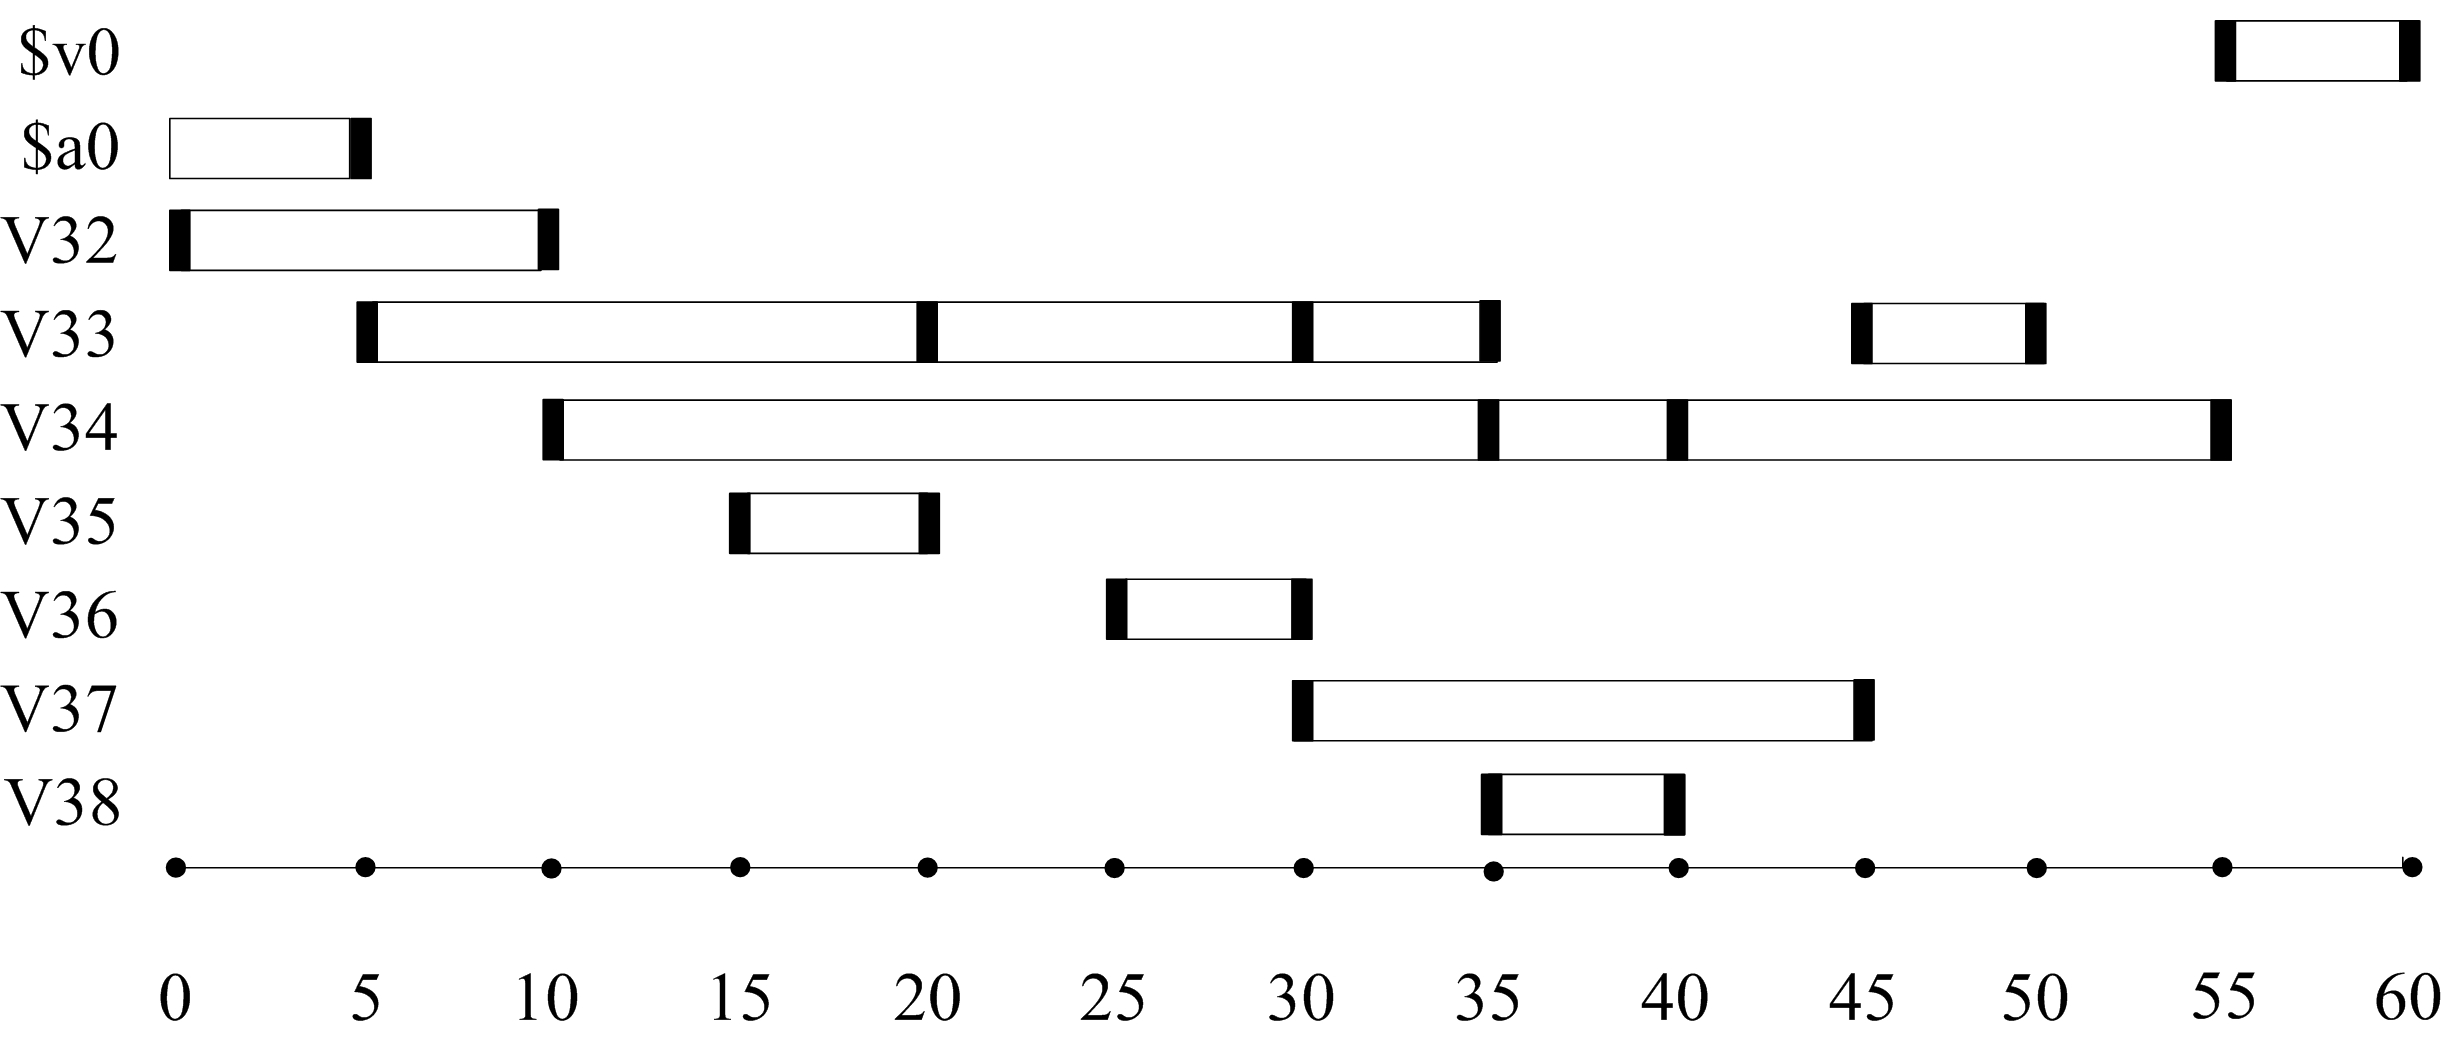
\includegraphics[scale=0.6]{{figures/figure07.02}.jpg}}
\end{center}

\bigskip

The numbers on the horizontal axis represent instruction ids and the vertical axis is labeled with register IDs

\bigskip

The darker vertical segments in the intervals identify use positions: a use position is a position in the interval where either the register is defined (ie, written) or the register is being used (ie, read)
\end{frame}

\begin{frame}[fragile]
\pause

We first compute, for each block, two local liveness sets: liveUse and liveDef

\pause
\bigskip

LiveUse operands are those operands that are read (or used) before they are written (defined) in the block's instruction sequence

\pause
\bigskip

LiveDef operands are those operands that are written to (defined) by some instruction in the block

\pause

\begin{algorithm}[H]
\begin{algorithmic}
\REQUIRE The control-flow graph $g$ for a method
\ENSURE Two sets for each basic block: liveUse, registers used before they are overwritten (defined) in the block and liveDef, registers that are defined in the block
\FOR {block $b$ in $g$.blocks}
\STATE Set $b$.liveUse $ \gets \{\}$
\STATE Set $b$.liveDef $ \gets \{\}$
\FOR {instruction $i$ in $b$.instructions}
\FOR {virtual register $v$ in $i$.readOperands}
\IF {$v \notin b$.liveDef}
\STATE $b$.liveUse.add($v$) 
\ENDIF
\ENDFOR
\FOR {virtual register $v$ in $i$.writeOperands}
\STATE $b$.liveDef.add($v$)
\ENDFOR
\ENDFOR
\ENDFOR
\end{algorithmic}
\caption{Computing Local Liveness Information}\index{liveness sets!local|(}
\end{algorithm}
\end{frame}

\begin{frame}[fragile]
\pause

The control-flow graph for \lstinline{Factorial.computeIter()} with its local liveness sets computed is illustrated below
\begin{center}
\visible<2->{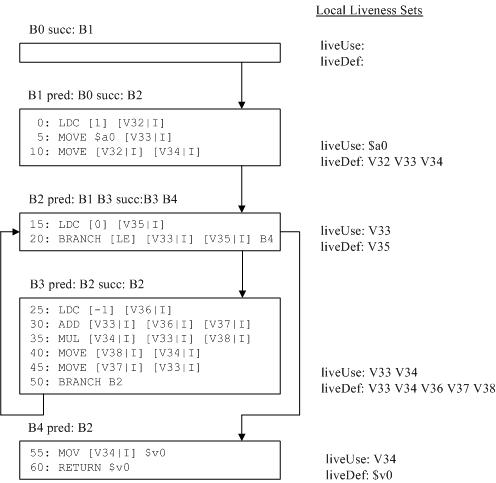
\includegraphics[scale=0.6]{{figures/figure07.03}.jpg}}
\end{center}
\end{frame}

\begin{frame}[fragile]
\pause

We can compute the set of operands that are live at the beginning and end of a block
using a backward data-flow analysis

\pause
\bigskip

We call the set of operands that are live at the start of a block liveIn

\pause
\bigskip

We call the set of operands that are live at the end of a block liveOut

\pause

\begin{algorithm}[H]
\begin{algorithmic}
\REQUIRE The control-flow graph $g$ for a method, and the local liveness sets liveUse and liveDef for every basic block
\ENSURE Two sets for each basic block: liveIn, registers live at the beginning of the block, and liveOut, registers that are live at the end of the block
\REPEAT
    \FOR {block $b$ in $g$.blocks in reverse order}
        \STATE $b$.liveOut $ \gets \{\} $
        \FOR {block $s$ in $b$.successors}
            \STATE $b$.liveOut $\gets$ $b$.liveOut $\cup$ $s$.liveIn
        \ENDFOR
        \STATE $b$.liveIn $\gets$  ($b$.liveOut $-$  $b$.liveDef) $\cup$  $b$.liveUse
    \ENDFOR
\UNTIL{ no liveOut has changed }

\end{algorithmic}
\caption{Computing Global Liveness Information}
\end{algorithm}
\end{frame}

\begin{frame}[fragile]
\pause

The computation of the global liveness information for \lstinline{Factorial.computeIter()} requires three iterations

\pause
\bigskip

After first iteration
\begin{lstlisting}[language={}]
B4 liveIn:  V34
B4 liveOut:
B3 liveIn:  V33 V34
B3 liveOut:
B2 liveIn:  V33 V34
B2 liveOut: V33 V34
B1 liveIn:  $a0                                                                 
B1 liveOut: V33 V34                                                             
B0 liveIn:  $a0
B0 liveOut: $a0
\end{lstlisting}

\pause

After second iteration
\begin{lstlisting}[language={}]
B4 liveIn:  V34
B4 liveOut:
B3 liveIn:  V33 V34
B3 liveOut: V33 V34
B2 liveIn:  V33 V34
B2 liveOut: V33 V34
B1 liveIn:  $a0                                                                 
B1 liveOut: V33 V34                                                             
B0 liveIn:  $a0
B0 liveOut: $a0
\end{lstlisting}
\end{frame}

\begin{frame}[fragile]
\pause

After third (and final) iteration
\begin{lstlisting}[language={}]
B4 liveIn:  V34
B4 liveOut:
B3 liveIn:  V33 V34
B3 liveOut: V33 V34
B2 liveIn:  V33 V34
B2 liveOut: V33 V34
B1 liveIn:  $a0
B1 liveOut: V33 V34
B0 liveIn:  $a0                                                                 
B0 liveOut: $a0
\end{lstlisting}
\end{frame}
\end{document}
